\section{Polychromatic Correction Temperature Fit Residual Data Plots}
%=====================================================================
\label{app.tfit_data_plots}
%\newpage

\addcontentsline{toc}{subsection}{Channels 1-6}
\begin{figure}[H]
  \centering
  \begin{tabular}{c c}
    \includegraphics[scale=0.35]{graphics/tfit/gmi_gpm-1.tfit.eps} &
    \includegraphics[scale=0.35]{graphics/tfit/gmi_gpm-2.tfit.eps} \\\\
    \includegraphics[scale=0.35]{graphics/tfit/gmi_gpm-3.tfit.eps} &
    \includegraphics[scale=0.35]{graphics/tfit/gmi_gpm-4.tfit.eps} \\\\
    \includegraphics[scale=0.35]{graphics/tfit/gmi_gpm-5.tfit.eps} &
    \includegraphics[scale=0.35]{graphics/tfit/gmi_gpm-6.tfit.eps} \\
  \end{tabular}
  \caption{GMI channels 1-6 polychromatic correction temperature fit residuals for the three test temperatures: $T_{NOM}$ (25\textdegree{}C), $T_{LO}$ (-10\textdegree{}C), and $T_{HI}$ (45\textdegree{}C).}
  \label{fig:ch1-6_tfit}
\end{figure}

\addcontentsline{toc}{subsection}{Channels 7-12}
\begin{figure}[H]
  \centering
  \begin{tabular}{c c}
    \includegraphics[scale=0.35]{graphics/tfit/gmi_gpm-7.tfit.eps} &
    \includegraphics[scale=0.35]{graphics/tfit/gmi_gpm-8.tfit.eps} \\\\
    \includegraphics[scale=0.35]{graphics/tfit/gmi_gpm-9.tfit.eps} &
    \includegraphics[scale=0.35]{graphics/tfit/gmi_gpm-10.tfit.eps} \\\\
    \includegraphics[scale=0.35]{graphics/tfit/gmi_gpm-11.tfit.eps} &
    \includegraphics[scale=0.35]{graphics/tfit/gmi_gpm-12.tfit.eps} \\
  \end{tabular}
  \caption{GMI channels 7-12 polychromatic correction temperature fit residuals for the three test temperatures: $T_{NOM}$ (25\textdegree{}C), $T_{LO}$ (-10\textdegree{}C), and $T_{HI}$ (45\textdegree{}C).}
  \label{fig:ch7-12_tfit}
\end{figure}

\addcontentsline{toc}{subsection}{Channel 13}
\begin{figure}[H]
  \centering
  \includegraphics[scale=0.35]{graphics/tfit/gmi_gpm-13.tfit.eps}
  \caption{GMI channel 13 polychromatic correction temperature fit residuals for the three test temperatures: $T_{NOM}$ (25\textdegree{}C), $T_{LO}$ (-10\textdegree{}C), and $T_{HI}$ (45\textdegree{}C).}
  \label{fig:ch13_tfit}
\end{figure}

